\documentclass{standalone}
\usepackage{tikz}
\usetikzlibrary{arrows,positioning}
\begin{document}

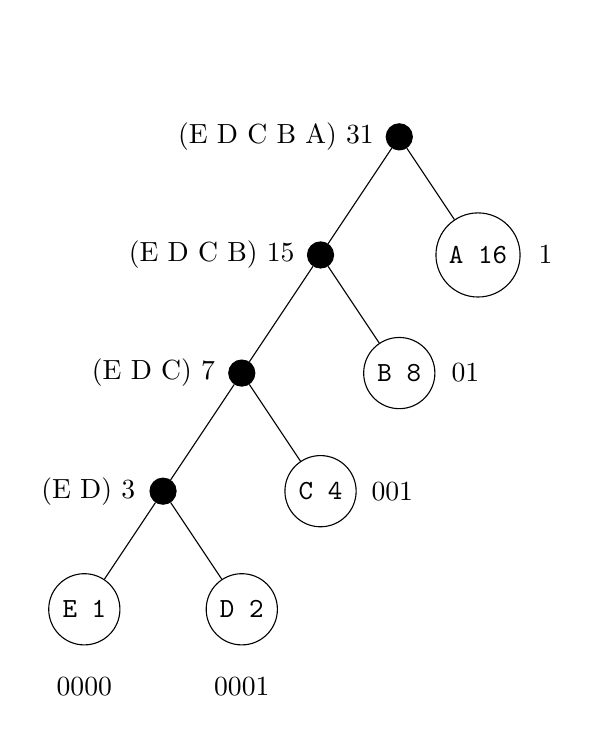
\begin{tikzpicture}[
	level 1/.style = {sibling distance=20mm},
	every node/.style = {draw, circle, fill=black},
	leaf/.style = {draw, circle, minimum size = 5mm, fill=none}
]
\node [label=left:(E D C B A) 31] {}
	child {node [label=left:(E D C B) 15] {}
		child {node [label=left:(E D C) 7] {}
			child {node [label=left:(E D) 3] {}
				child {node [leaf] [label=below:0000] {\texttt{E 1}}}
				child {node [leaf] [label=below:0001] {\texttt{D 2}}}}
			child {node [label=right:001] [leaf] {\texttt{C 4}}}}
		child {node [label=right:01] [leaf] {\texttt{B 8}}}}
	child {node [label=right:1] [leaf] {\texttt{A 16}}};
\end{tikzpicture}

\end{document}
